\documentclass[11pt,a4paper]{article}
\usepackage[utf8]{inputenc}
\usepackage[czech]{babel}
%\usepackage{amsfonts}
%\usepackage{amsthm}
%\usepackage{amsmath}
%\usepackage{amssymb}
\usepackage[pdftex]{graphicx}
%\usepackage{enumerate}
%\usepackage{stmaryrd}
\usepackage{hyperref}

%\newtheorem{tvrz}{Tvrzení}
%\newtheorem{uloh}{Úloha}
%\newtheorem{lem}[tvrz]{Lemma}

\newcommand{\HRule}{\rule{\linewidth}{0.5mm}}

\begin{document}

\begin{titlepage}
\begin{center}
% Upper part of the page

\includegraphics[viewport=180 50 100 100,scale=0.5]{./logo_mff.jpg}\\[1cm]    

\textsc{\LARGE Matematicko-fyzikální fakulta\\[0.1cm]
Univerzity Karlovy v Praze}\\[1.5cm]

\textsc{\Large Zápočtový program k NPRG030\\ ZS 2010/2011}\\[0.5cm]


% Title
\HRule \\[0.4cm]
{ \huge \bfseries Knihovna twhree}\\[0.4cm]

\HRule \\[1.5cm]

% Author and supervisor
\begin{minipage}{0.4\textwidth}
\begin{flushleft} \large
\emph{Autor:}\\
Duc Trung \textsc{Ha}
\end{flushleft}
\end{minipage}
\begin{minipage}{0.4\textwidth}
\begin{flushright} \large
\emph{Cvičící:} \\
Bc.~Jan \textsc{Kohout}
\end{flushright}
\end{minipage}

\vfill
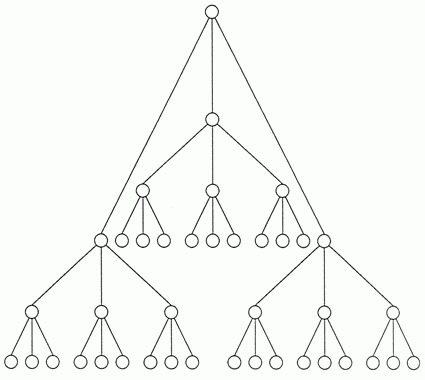
\includegraphics[viewport=330 50 100 100,scale=0.5]{./tree.jpg}\\[1cm]    

% Bottom of the page
{\large \today}

\end{center}

\end{titlepage}

\begin{abstract}
Dokumentace k zápočtovému programu.
Program je implementací datové struktury binárního vyhledávacího 2-3 stromu a
základních operací na něm.
\end{abstract}

\pagebreak

\tableofcontents

\pagebreak

\part{Úvodní slovo}
Informační doba si žádá v~čím dál větší míře lepší a lepší organizaci a
zpracování dat.
Gigantické databáze s astronomickým množstvím dat již dnes nejsou žádnou
zvláštností.
Vyvstává přirozeně otázka, po jakých datových strukturách pro tento účel
sáhnout.

První, co většině lidí přijde na mysl, je využít pole či lineární spojové
seznamy, jež jsou jednodušše implementovatelné.
Tento přístup je ovšem poněkud naivní, neboť (ač vkládání lze zvládat v
konstantním čase) operace vyhledávání obnáší časovou nářočnost
$\mathcal{O}(n)$. 
Na tom není vůbec nic ošklivého, algoritmy polynomiální časové třídy jsou
obecně považovány za~e\-fektivní, ovšem pro účely databázových systémů, jež mají
často velikosti v~řádech miliard, to není zrovna nejvhodnější návrh. 

Na úkor vkládání lze však tento nesnadný úkol vyhledávání \uv{jehly v~kupce
sena} zvládnout pomocí sofistikovaných datových struktur v~krásném čase
$\mathcal{O}(\log n)$.

Jednou z takovýchto struktur je právě 2-3 strom, jehož standardní operace
(Insert, Delete, Find, Find Max, Find Min, Previous, Next) právě kni\-hovna
\textit{twhree} (jejíž název vznikl ze slov \textbf{T}wo-t\textbf{H}ree
t\textbf{REE}) implementuje.

\pagebreak

\part{Programátorský manuál}
\section{Anotace}
Implementace operací s vyváženými vyhledávacími stromy (např. AVL,
červe\-no-černými nebo 2-3): insert, delete, find, findmin, findmax, next. 

\section{Přesné zadání}
Implementujte datovou strukturu 2-3 stromu a jeho operací.
Strom bude obsahovat uzly dvojího typu:

\renewcommand{\labelitemi}{$\spadesuit$}

\begin{itemize}
\item \textbf{Vnitřní uzel} obsahující informace o svých podstromech a jejich
přísluš\-ných maximálních klíčů
\item \textbf{List} obsahující ukazatel na samotná data
\end{itemize}

Dále bude se stromem možné provádět následující operace:

\renewcommand{\labelitemi}{$\clubsuit$}

\begin{itemize}
\item \textbf{Insert} vkládající nový uzel do stromu s příslušným ukazatelem na
nově vytvořenou datovou položku
\item \textbf{Delete} mazající uzel se zadaným klíčem ze stromu spolu s jeho
přísluš\-nou datovou položku
\item \textbf{Find} vyhledávající uzel se zadaným klíčem ve stromu a vracející
ukazatel na danou datovou položku
\item \textbf{Findmin} vyhledávající uzel s nejnižším klíčem ve stromu a vracející
ukazatel na danou datovou položku
\item \textbf{Findmax} vyhledávající uzel s nejvyšším klíčem ve stromu a vracející
ukazatel na danou datovou položku
\item \textbf{Previous}\footnote{Lze si povšimnout, že oproti původnímu plánu
byla přidána operace \verb~Previous~, jež vyvstala jako logický důsledek
implementace operace \verb~Next~.}
vyhledávající uzel s nejbližší nižší hodnotou klíče ve stromu a vracející
ukazatel na danou datovou položku
\item \textbf{Next} vyhledávající uzel s nejbližší vyšší hodnotou klíče ve
stromu a~vracející ukazatel na danou datovou položku
\end{itemize}

\section{Algoritmy a datové struktury}
\subsection{Použité datové struktury}
V této sekci si přiblížíme použité datové části v programu.

\begin{tabular}{ | c || r | l | p{4cm} | }
  \hline
  \textbf{Hlavní} & \textbf{Datový} & \textbf{Název} & \textbf{Popis} \\
  \textbf{struktura} & \textbf{typ položky} & \textbf{položky} & \\
  \hline \hline
  TItem & int & key & \textit{klíč dat} \\
  & char [10] & name & \textit{samotná data - zde text} \\ 
  \hline \hline
  subtree & struct node * & sub & \textit{ukazatel na (pod)strom} \\
  & int & max\_key & \textit{...a příslušný klíč maximální velikosti} \\ 
  \hline \hline
  node & struct node * & parent & \textit{ukazatel na otce/rodiče uzlu} \\
  & subtree [3] & kidz & \textit{pole ukazatelů na potomky uzlu a jejich maximálních klíčů} \\ 
  & TItem * & pData & \textit{ukazatel na samotná data (pouze v uzlech)} \\
  \hline
\end{tabular}

Zřejmě nejzajímavější je položka \verb=kidz=, která reprezentuje 2 až 3 potomky uzlu.
Tato je řešena skrze pole z příčin ryze praktických $\Leftarrow$ snadnější
přerovnávání potomků pouhým jednoduchým zabublaním nověho přidaného prvku
z~pravého konce pole na vhodné místo (přitom potomek s hodnotou \verb=NULL=
položky \verb=sub= se vždy odsouvá napravo).

\subsection{Použité algoritmy}
V této sekci si popíšeme algoritmy použité na implementaci jednotlivých
operací na 2-3 stromech.
Půjde spíše o \uv{nošení dříví do lesa}, autoři 2-3 stromu totiž tyto algoritmy
navrhli s co možná největší efektivitou a proto není třeba vymýšlet něco nového
či převratného.

\subsubsection{Napojení knihovny na program}
Knihovna \verb=twhree= je psána v jazyku C a její integrování do programu je
velice jednoduché.
Soubory knihovny \verb=twhree.h= a \verb=twhree.c= stačí zkopírovat do složky s
programem využívajích této knihovny a do programu vložit následující řádek:

\begin{verbatim}
#include "twhree.h"
\end{verbatim}

To nalinkuje hlavičky funkcí a datové struktury knihovny.
Dál je nutné při kompilaci zkompilovat soubory knihovny a připojit je ke
kompilovanému programu.\footnote{Jako příklad tohoto může posloužit přiložený
\verb~Makefile~}

\subsubsection{Funkce insert}

Funkce má následující hlavičku:

\begin{verbatim}
struct node*
 insert(struct TItem *pNewItem, struct node **pRoot);
\end{verbatim}

Povšimněme si, že tato funkce přijímá jako argument ukazatel na ukazetel, tedy
\verb~struct node **~.
To je z toho důvodu, že potřebujeme měnit přímo ukazatel na kořen stromu
(bude-li na konci přidání jiný), a nestačí nám tedy měnit jen pouhá data
samotná, páč ty už nemusí být kořenem.

Dále funkce \verb~insert~ vrací ukazatel na nově přidaný uzel, to je čistě pro účely obslužného programu, aby dokázal vypsat informace o novém uzlu.
V případě potřeby lze přetypovat funkci na typ \verb~void~ a tím tuto drobnost vyřešit.

Jak ale samotný algoritmus pracuje?

Nejdřív jsou řešeny obskurní a málo časté speciální případy:

\renewcommand{\labelitemi}{$\sharp$}

\begin{itemize}
\item Strom je \textbf{prázdný}.
Pak se prostě vytvoří nový uzel s ukazatelem na daná data a označí se jako
jediný uzel stromu (tj. jako kořen).
\item Strom má \textbf{právě 1 uzel}.
Pak se vytvoří nový uzel s ukazatelem na daná data.
Dále se alokuje ještě společný rodič tohoto nového uzlu původního jediného
uzlu, jenž bude sloužit jako nový kořen stromu se potřebnými 2 potomky.
\item Jinak vznikají zajímavější případy.
Nejprve se nalezne vhodný interval klíčů, do kterého nová data podle svého
klíče zapadnou.
Hledáme vlastně vhodného rodiče nějakých listů, jejichž hodnoty klíčů již
určují, kam nový uzel zapadne.\footnote{Probíhá velmi podobně jako u funkce
\verb~find~ - vyhledá se dle klíčů a rozhoduje se dle toho, kterou větví
potomků se vydat}
Nyní se rozhoduje na základě toho, zda-li je pro nový uzel \uv{místo} v rodiči
dle pravidel 2-3 stromu.
  \renewcommand{\labelitemii}{$\Xi$}
  \begin{itemize}
  \item Rodič má \textbf{právě 2 potomky}.
  Pak se jednoduše na konec pole potomků přidá tento nový uzel a ten se posléze
  díky funkci \verb~BubleKidz~ zarovná (konkrétně \uv{zabublá}) na správné
  místo.
  \item Rodič má \textbf{právě 3 potomky}.
  Nejprve se stejnak vytvoří daný nový uzel.
  Pak se rozdělí dotyčný rodič na 2 uzly\footnote{Konkrétně se vytvoří nový
  pravý sourozenec tohoto rodiče} a mezi ně se rozdělí tito 4 potomci v poměru
  2 a 2, přičemž se zachová vzestupné pořadí klíčů.\footnote{Ty se seřadí v
  pomocném poli \verb~tmp\_kidz\[\]~}

  Pokud rodič těchto 2 rozdělených uzlů\footnote{tj. rodič nalezeného rodiče}
  má nyní nanejvýš 3 potomky je vše v pořádku a s \verb~insert~ může vrátit
  požadovaný ukazatel na uzel s nově vkládanými daty (viz výše).

  Pokud rodič těchto 2 rozdělených uzlů má nyní 4, postupuje se pro něj
  analogicky rekursivně.\footnote{tj. vytvoří se jeho pravý sourozenec a jeho 4
  potomci se mezi tyto 2 rodiče rozdělí po dvou}
  \end{itemize}
\end{itemize}

Je ještě důležité nezapomenout aktualizovat hodnoty maximálních klíčů u předků
nově vkládaných uzlů.
Pokud se totiž uzlu přidá nový (úplně \uv{nejpravější}) potomek, změní se tím
samozřejmě i hodnota největšího klíče podstromu s kořenem v tomto uzlu.

\subsubsection{Funkce delete}

Funkce má následující hlavičku:

\begin{verbatim}
int delete(struct node **pRoot, int key);
\end{verbatim}

V atributu \verb~key~ přijímá klíč k vyhledání mazaného listu.

Pokud list s klíčem není nalezen, funkce vrací hodnotu $1$ či $-1$ (v případě
prázdného stromu).

Pokud list s klíčem nalezen je, funkce vrací hodnotu $0$.
Algoritmus přitom maže list následujícím způsobem:

\renewcommand{\labelitemi}{$\Theta$}
\begin{itemize}
\item Je-li uzel jediný ve stromu, tj. jedná se o samostatný \textbf{kořen},
jednoduše se dealokuje společně s daty, na něž ukazuje.
\item Má-li rodič uzlu \textbf{3 potomky}, jednoduše se uzel smaže, v rodiči
se patřičně setřídí vzestupně klíče a upraví se hodnoty maximálních klíčů pro
další předky.\footnote{V případě, že jsme smazali něčí maximální klíč.}
\item Má-li rodič uzlu \textbf{2 potomky}, rozlišují se následující 3 případy:

  \renewcommand{\labelitemii}{$\Upsilon$}
  \begin{itemize}
  \item Je-li rodič \textit{kořenem stromu}, uzel se smaže a za nový kořen
  stromu se určí jeho sourozenec.
  \item Má-li rodič nějakého \textit{sourozence se 3 potomky}, jednoho si
  \uv{ukradne} pro vyrovnání počtu vlastních dětí.\footnote{Tedy zabitý uzel je
  nahrazen tak, že jeho rodič místo něj adoptuje jeho bratrance z početnější
  rodinky {\tt :-)}}
  \item Má-li rodič jen \textit{sourozence se 2 potomky}, jednomu z nich
  přenechá svého jediného zbývajícího syna, čímž ze sourozence udělá uzel se 3
  potomky.
  Ovšem nyní se musí eliminovat uzel s rodičem smazaného uzlu.
  Není nic jednoduššího-prostě se i na něj rekursivně zavolá funkce pro smazání
  uzlu, a pokud bychom takto rekursí náhodou došlu až ke kořeni, kořenový uzel
  se prostě smaže a kořen se přenastaví, jak je to popsáno o 2 body výše.
  \end{itemize}

\end{itemize}

\subsubsection{Funkce find}

Tato funkce má následující podobu:

\begin{verbatim}
struct TItem * find(struct node *root, int sKey);
\end{verbatim}

Rozhoduje se podle těchto 3 situací:

\renewcommand{\labelitemi}{$\nabla$}

\begin{itemize}
\item V případě \textbf{prázdného stromu} vrací ukazatel \verb~NULL~.
\item V případě \textbf{listu} obsahující hledaný klíč vrací ukazatel na svá data.
\item V případě \textbf{listu} NEobsahující hledaný klíč vrací ukazatel
\verb~NULL~ (tj. položka s daným klíčem nebyla nalezena).
\item V případě \textbf{vnitřního uzlu} se rekursivně předá hledání do 1 z potomků.
Přitom se rozhoduje dle hodnot maximálních klíčů podstromů.
Ty vlastně rozdělují hodnoty klíčů na intervaly a podle toho, kam hledaný klíč
spadne, rozhodne se o cestě dál.
\end{itemize}

\subsubsection{Funkce findMin}

Tato funkce má tuto hlavičku:

\begin{verbatim}
struct TItem * findMin(struct node *root);
\end{verbatim}

Její algoritmus je vskutku jednoduchý: z vrcholu se vydavá vždy do 1. potomku
(nejvíc vlevo), dokud nedorazí do listu (ty jsou všechny ve stejné výšce, a
jelikož jsou na této úrovni již seřazeni, nalezne se skutečně nejmenší).

\subsubsection{Funkce findMax}

Tato funkce má takovouto hlavičku:

\begin{verbatim}
struct TItem * findMax(struct node *root);
\end{verbatim}

Její algoritmus je velice podobný funkci \verb~findMin~: z vrcholu se vydavá
vždy do 3. potomku či (pokud ho nemá) do 2. potomku (tj. nejvíc napravo), dokud
nedorazí do listu.

\subsubsection{Funkce previous}

Funkce s následující hlavičkou:

\begin{verbatim}
struct TItem * previous(struct node *root, int sKey);
\end{verbatim}

Algoritmus nejprve nalezne uzel s daným klíčem (pokud neexistuje, vratí
\verb~NULL~), potom se snaží najít jeho nejbližšího levého sourozence.

Pokud ho nenalezne, postoupí ke svému rodiči \uv{nahoru} a tam se rekursivně
opět pokusí najít nejbližšího levého sourozence.

Pokud ho nalezne, vrací maximum podstromu tohoto sourozence.\footnote{s
využítím funkce \verb~findMax~ - viz výše} To odpovídá tomu, že chceme najít
největší klíč, který je menší než ten zadaný.

Pokud dorazí až do kořene stromu, nemůže dál a znamená to, že zadaný klíč byl
ve stromu nejmenší.

\subsubsection{Funkce next}

Funkce s následující hlavičkou:

\begin{verbatim}
struct TItem * next(struct node *root, int sKey);
\end{verbatim}

Opět zcela analogicky algoritmus nejprve nalezne uzel s daným klíčem (pokud
neexistuje, vratí \verb~NULL~), potom se snaží najít jeho nejbližšího pravého
sourozence.
Vše je opravdu podobné funkci \verb~previous~ jen s tím rozdílem, že se hledá
pravý sourozenec a pak se spustí \verb~findMin~.

\pagebreak

\part{Uživatelský manuál}
Pro účely názorné demonstrace knihovny \textit{twhree} byl sepsán obslužný
program umístěný v souboru \verb=main.c=.
Ten je zcela separován od knihovních funkcí, tudíž ho lze použít
na~demonstrace jiných stromů.
Naopak i knihovnu \textit{twhree} lze univerzálně užívat v jiných programech.
Pro ukázku práce s touto obsluhou zde bude zobrazeno několik výstupů z
obrazovky a způsobu zadávání příslušných vstupních dat.

\section{Menu}
Při spuštění obsluhy nás uvítá zpráva o aktuální verzi ovládacího programu:

\begin{verbatim}
Welcome to twhree v2.3!
This is a demonstration program of twhree [T(wo)-(t)H(ree)
(t)REE] library.
\end{verbatim}

Následuje nabídka příkazů:

\begin{verbatim}
------------------------------------------------------------------
Choose option (enter the part in brackets)
(I)nsert         - insert a new node 
(D)elete         - delete the node containing specified value 
delete (A)ll     - delete the node containing specified value 
(F)ind           - ascertain the presence of the value in the tree 
find(M)in        - show the minimum of the tree 
findma(X)        - show the maximum of the tree 
(P)revious       - show the previous item according to the key 
(N)ext           - show the next item according to the key 
displa(Y)        - display tree (depth-first, preorder) 
c(L)ear          - clear screen (only for in *nix like OS) 
(H)elp           - displays this menu:) 
(Q)uit           - quit the program 
------------------------------------------------------------------
>> 
\end{verbatim}

Jak vidno, tuto nabídku lze kdykolit znova vyvolat pomocí
příkazu\footnote{Příkazy lze zadávat velkými i malými písmeny abecedy.
Dokonce ani nevadí, když jsou za prvním písmenem další znaky, ty se do konce
řádku ignorují.} \verb=h=:

\begin{verbatim}
>> h 
\end{verbatim}

\section{Vstup a příkazy programu}
\subsection{Insert}
Příkaz vložení nové položky se zadaným klíčem a textem (reprezentující data).
Na tu pak ve stromu ukazuje nově vkládaný uzel.

\begin{verbatim}
>> i
Enter new item...
 New key: 1
 New name: aaa
Adding "aaa" with key 1......OK
\end{verbatim}

\subsection{Delete}
Příkaz smazání položky se zadaným klíčem včetně k ní příslušného uzlu
ve~stromu.

\begin{verbatim}
>> d
 Which key: 1
Deleting node with key 1......OK
\end{verbatim}

V případě nenalezení zadaného klíče:

\begin{verbatim}
>> d
 Which key: -1
Deleting node with key -1......KEY NOT FOUND!
\end{verbatim}

Je-li dokonce strom prázdný:

\begin{verbatim}
>> d
 Which key: -1
Deleting node with key -1......EMPTY TREE!
\end{verbatim}

\subsection{Delete all}
Příkaz smazání všech položek a tím i celého stromu.\footnote{Mimochodem tento
příkaz se defaultně volá při ukončení programu, neb data nejsou ukládána
externě do souboru na disku, nýbrž jsou zachovávána interně v hlavní paměti
počítače a tam po skončení práce pak jen zabírají zbytečně místo.}

\begin{verbatim}
>> a
\end{verbatim}

\subsection{Find}
Příkaz vyhledání položky se zadaným klíčem.

\begin{verbatim}
>> f
 Search key: 1
Serching key 1...... (1,"aaa")
\end{verbatim}

V případě nenalezení zadaného klíče:

\begin{verbatim}
>> f
 Search key: -1
Serching key -1......NOT FOUND!
\end{verbatim}

\subsection{Find min}
Příkaz vyhledání položky se nejmenším klíčem.\footnotemark[4]

\begin{verbatim}
>> m
Searching minimal key...... (1,"1")
\end{verbatim}

\subsection{Find max}
Příkaz vyhledání položky se největším klíčem.\footnote{V případě existence více
takových položek nalezne tu, jež byla přidána první. To by se nemělo stávat,
neboť klíče by měly být v databázích unikátní - možná bude předmětem zájmu v
dalších verzích.}

\begin{verbatim}
>> x
Searching maximal key...... (1,"1")
\end{verbatim}

\subsection{Previous}
Příkaz vyhledání položky s nejbližší nižší hodnotou klíče.

\begin{verbatim}
>> p
 Previous of which key? 2
Searching previous item of item with 2 key...... (1,"aaa")
\end{verbatim}

\subsection{Next}
Příkaz vyhledání položky s nejbližší vyšší hodnotou klíče.

\begin{verbatim}
>> n
 Next of which key? 0
Searching next item of item with 0 key...... (1,"aaa")
\end{verbatim}

\subsection{Display}
Příkaz zobrazení 2-3 stromu.
Každá hlubší úroveň stromu je o 1 mezeru více odsazená než předchozí,
bezprostředně vždy následují potomci aktuálního uzlu (a popř. jejich potomci s
příslušným odsazením).
Vnitřní uzly jsou v~[hranatých závorkách] spolu s maximálními klíčemi levého
popř. prostřední\-ho stromu, listy zas v (kulatých závorkách) s klíčem a hodnotou
dat příslušné položky:

\begin{verbatim}
>> y
[4]
 [2]
  [1]
   (1,"a")
   (2,"b")
  [3]
   (3,"c")
   (4,"d")
 [6|8]
  [5]
   (5,"e")
   (6,"g")
  [7]
   (7,"f")
   (8,"h")
  [9|10]
   (9,"k")
   (10,"l")
   (11,"j")
\end{verbatim}

\subsection{Clear}
Příkaz na vyčištění obrazovky (v abstraktním slova smyslu, samozřejmě, jinak
použijte suchý hadřík či látku {\tt :-)}
Funguje převážně na systémech *nixového typu, páč využívá systémové procedury
\verb=clear=.

\begin{verbatim}
>> l
\end{verbatim}

\subsection{Quit}
A tady končí naše cesta...

\begin{verbatim}
>> q
Bye bye...
\end{verbatim}

\pagebreak

\begin{thebibliography}{9}

\bibitem{wiki-2-3-tree}
\url{http://en.wikipedia.org/wiki/2-3_tree}

\bibitem{cs-wisc-edu}
\url{http://pages.cs.wisc.edu/~vernon/cs367/notes/10.23TREE.html}

\bibitem{topfer-knizka}
Doc.~RNDr.~T\"opfer, Pavel. \textsl{Algoritmy a programovací techniky},
2.~vydání, Prometheus, Praha (2007). ISBN 978-80-7196-350-9.

\end{thebibliography}

\end{document}
